\documentclass[border=4pt]{standalone}
\usepackage{tikz}
\usepackage{amsmath}
\usetikzlibrary{arrows.meta,calc,positioning}
\begin{document}
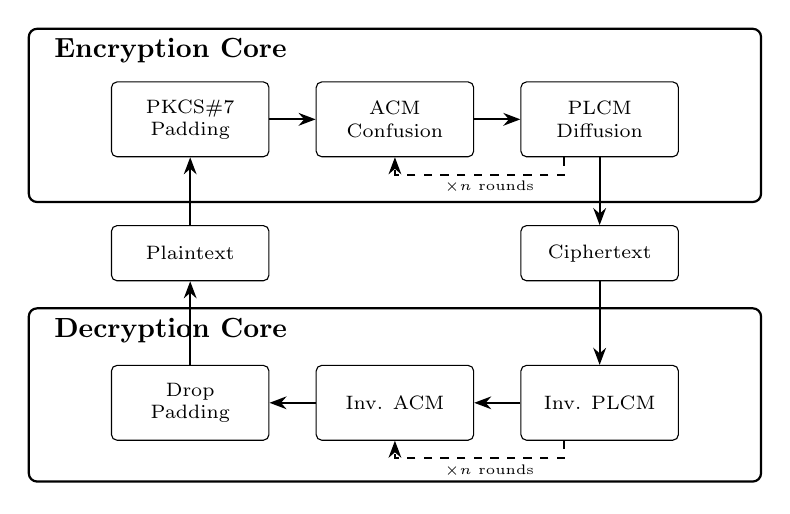
\begin{tikzpicture}[
    >=Stealth,
    font=\scriptsize,
    arr/.style={->, line width=0.7pt},
    darr/.style={->, dashed, line width=0.7pt},
    frame/.style={draw, rounded corners=3pt, line width=0.8pt},
    mbox/.style={draw, rounded corners=2pt, align=center, inner sep=3pt,
                 minimum width=2.0cm, minimum height=0.95cm},
    bridge/.style={draw, rounded corners=2pt, align=center,
                   minimum width=2.0cm, minimum height=0.7cm},
    note/.style={font=\tiny, align=center}
]

% ---- shared column x-positions ----
\def\cA{2.4}
\def\cB{5.0}
\def\cC{7.6}

% ---- row y-positions (boxes lowered inside frames) ----
\def\rEnc{-1.55}
\def\rBridge{-3.25}
\def\rDec{-5.15}

% frame vertical extents
\def\encTop{-0.4}
\def\encBot{-2.6}
\def\decTop{-3.95}
\def\decBot{-6.15}

% ===== ENCRYPTION CORE =====
\draw[frame] (0.35,\encTop) rectangle (9.65,\encBot);
\node[anchor=west, font=\bfseries\normalsize] at (0.55,-0.68) {Encryption Core};

\node[mbox] (epad)  at (\cA,\rEnc) {PKCS\#7\\Padding};
\node[mbox] (eacm)  at (\cB,\rEnc) {ACM\\Confusion};
\node[mbox] (eplcm) at (\cC,\rEnc) {PLCM\\Diffusion};

\draw[arr] (epad) -- (eacm);
\draw[arr] (eacm) -- (eplcm);
% feedback loop: tap PLCM slightly left of center so it doesn't collide
% with the downward ciphertext arrow (which leaves from PLCM's center-south)
\draw[darr] ($(eplcm.south)+(-0.45,0)$) -- ++(0,-0.22) -| (eacm.south);
\node[note] at ($(eacm.south)!0.5!(eplcm.south)+(-0.1,-0.38)$) {$\times n$ rounds};

% ===== DECRYPTION CORE =====
\draw[frame] (0.35,\decTop) rectangle (9.65,\decBot);
\node[anchor=west, font=\bfseries\normalsize] at (0.55,-4.23) {Decryption Core};

\node[mbox] (ddrop)  at (\cA,\rDec) {Drop\\Padding};
\node[mbox] (diacm)  at (\cB,\rDec) {Inv. ACM};
\node[mbox] (diplcm) at (\cC,\rDec) {Inv. PLCM};

\draw[arr] (diplcm) -- (diacm);
\draw[arr] (diacm) -- (ddrop);
\draw[darr] ($(diplcm.south)+(-0.45,0)$) -- ++(0,-0.22) -| (diacm.south);
\node[note] at ($(diacm.south)!0.5!(diplcm.south)+(-0.1,-0.38)$) {$\times n$ rounds};

% ===== BRIDGES =====
\node[bridge] (plain)  at (\cA,\rBridge) {Plaintext};
\node[bridge] (cipher) at (\cC,\rBridge) {Ciphertext};

% closed loop
\draw[arr] (plain.north)  -- (epad.south);
% ciphertext arrow leaves PLCM center-south, lands cipher top
\draw[arr] (eplcm.south)  -- (cipher.north);
\draw[arr] (cipher.south) -- (diplcm.north);
\draw[arr] (ddrop.north)  -- (plain.south);

\end{tikzpicture}
\end{document}